95. \begin{figure}[ht!]
\center{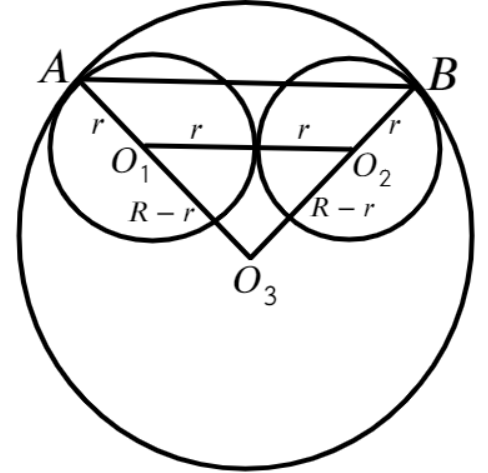
\includegraphics[scale=0.35]{g9-95.png}}
\end{figure}\\
Так как точки касания окружностей лежат на одной прямой с их центрами, имеем $O_1O_2=2r,$\\$O_1O_3=O_2O_3=R-r.$ Треугольники $O_1O_3O_2$ и $AO_3B$ подобны по двум сторонам и углу между ними (угол $O_3$ общий, $\cfrac{O_1O_3}{AO_3}=\cfrac{R-r}{R}=\cfrac{O_2O_3}{BO_3}),$ значит $\cfrac{10}{11}=\cfrac{R-5}{R},\ 10R=11R-55,\ R=55.$\\
